\documentclass[tikz,border=10pt]{standalone}
\begin{document}
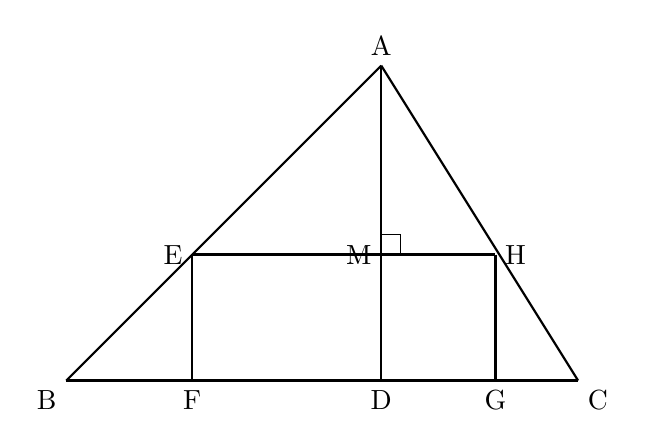
\begin{tikzpicture}[scale=1]
\coordinate (A) at (4,4);
\coordinate (B) at (0,0);
\coordinate (C) at (6.5,0);
\coordinate (D) at (4,0);
\coordinate (E) at (1.6,1.6);
\coordinate (F) at (1.6,0);
\coordinate (G) at (5.45,0);
\coordinate (H) at (5.45,1.6);
\coordinate (M) at (4,1.6);

\draw[thick] (B) -- (C);
\draw[thick] (A) -- (B);
\draw[thick] (A) -- (C);
\draw[thick] (A) -- (D);
\draw[thick] (E) -- (H);
\draw[thick] (E) -- (F);
\draw[thick] (H) -- (G);

% right angle mark at M
\draw (4.25,1.6) -- (4.25,1.85) -- (4,1.85);

\node[above] at (A) {A};
\node[below left] at (B) {B};
\node[below right] at (C) {C};
\node[below] at (D) {D};
\node[left] at (E) {E};
\node[below] at (F) {F};
\node[below] at (G) {G};
\node[right] at (H) {H};
\node[left] at (M) {M};
\end{tikzpicture}
\end{document}
